Betrachten Sie die Wahrscheinlichkeitsdichte
\[
\varphi(x)
=
\begin{cases}
0&\qquad  x \le -1        \\
a(1-x^2)&\qquad -1 <   x   \le 0 \\
a&\qquad  0 <   x   \le 1 \\
0&\qquad  1 < x
\end{cases}
\]
\begin{center}
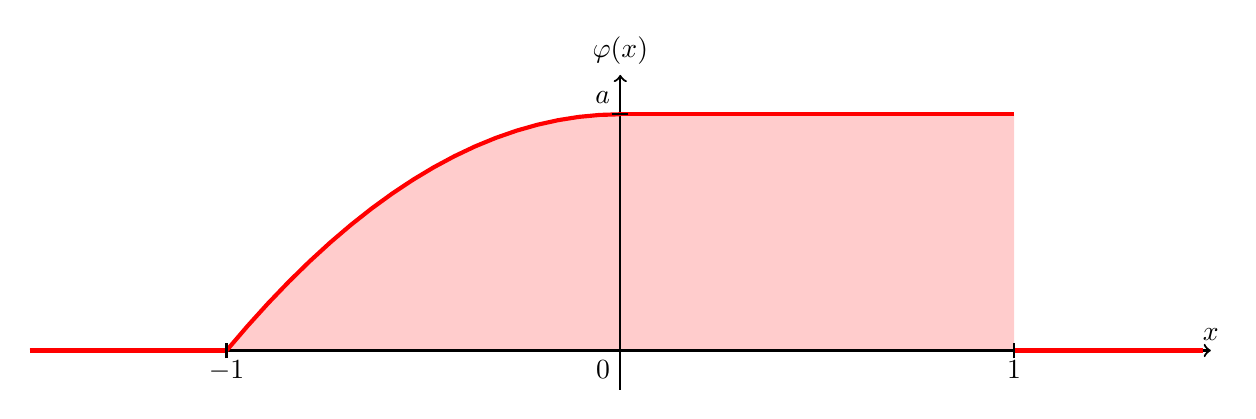
\begin{tikzpicture}[scale=5,thick]
\def\a{0.6}
\fill[color=red!20] (-1,0)--(1,0)--(1,{\a})--(0,{\a})--cycle;
\fill[color=red!20,domain=-1:0] plot ({\x},{\a*(1-\x*\x)})--(0,0)--cycle;
\draw[->] (-1.5,0)--(1.5,0) coordinate[label={$x$}];
\draw[->] (0,-0.1)--(0,{\a+0.1}) coordinate[label={$\varphi(x)$}];
\draw[color=red,line width=1.5pt] (-1.5,0)--(-1,0);
\draw[color=red,line width=1.5pt,domain=-1:0,samples=20] plot ({\x},{\a*(1-\x*\x)});
\draw[color=red,line width=1.5pt] (0,{\a})--(1,{\a});
\draw[color=red,line width=1.5pt] (1,0)--(1.48,0);
\draw (1,-0.02)--(1,0.02);	\node at (1,0) [below] {$1$};
\draw (-1,-0.02)--(-1,0.02);	\node at (-1,0) [below] {$-1$};
\draw (-0.02,{\a})--(0.02,{\a});	\node at (0,{\a}) [above left] {$a$};
\node at (0,0) [below left] {$0$};
\end{tikzpicture}
\end{center}
\begin{teilaufgaben}
\item Wie muss $a$ gewählt werden, damit $\varphi$ tatsächlich eine
Wahrscheinlichkeitsdichte ist?
\item Berechnen Sie den Erwartungswert einer Zufallsvariable mit dieser
Wahrscheinlichkeitsdichte.
\item Berechnen Sie die Varianz einer Zufallsvariable mit dieser
Wahrscheinlichkeitsdichte.
\end{teilaufgaben}

\thema{Wahrscheinlichkeitsdichte}
\thema{Erwartungswert}
\thema{Varianz}

\begin{loesung}
\begin{teilaufgaben}
\item
Die Normierung muss stimmen, d.~h.~es muss gelten
\begin{align*}
1=\int_{-\infty}^{\infty}\varphi(x)\,dx
&=
\int_{-1}^0 a(1-x^2)\,dx
+
\int_{0}^1 a\,dx
\\
&=
a\biggl[x-\frac{x^3}{3}\biggr]_{-1}^0
+
a\biggl[x\biggr]_0^1
=
a\biggl(\frac23+1\biggr)=a\cdot\frac53
\qquad\Rightarrow\qquad a=\frac35 = 0.6.
\end{align*}
\item
Der Erwartungswert ist
\begin{align*}
E(X)
&=
\int_{-\infty}^\infty x\,\varphi(x)\,dx
=
\int_{-1}^0 x\cdot a(1-x^2) \,dx
+
\int_0^1x\cdot a\,dx
=
a\biggl[\frac{x^2}2-\frac{x^4}4\biggr]_{-1}^0
+
a\biggl[\frac{x^2}2\biggr]_0^1
\\
&=
-a\frac14+a\frac12=a\frac14=\frac35\cdot\frac14=\frac{3}{20}=0.15.
\end{align*}
\item
Für die Varianz brauchen wir zusätzlich 
\begin{align*}
E(X^2)
&=
\int_{-\infty}^\infty x^2\,\varphi(x)\,dx
=
\int_{-1}^0 x^2\cdot a(1-x^2)\,dx
+
\int_0^1 x^2\cdot a\,dx
=
a\biggl[\frac{x^3}{3}-\frac{x^5}{5}\biggr]_{-1}^0
+
a\biggl[\frac{x^3}{3}\biggr]_0^1
\\
&=
a\biggl(-\frac2{15}+\frac13\biggr)
=
a\frac{7}{15}
=
\frac{3}{5}\cdot\frac{7}{15}
=
\frac{7}{25}=0.28.
\end{align*}
Damit können wir jetzt die Varianz ausrechnen:
\begin{align*}
\operatorname{var}(X)
&=
E(X^2)-E(X)^2
=
\frac{7}{25}-\biggl(\frac{3}{20}\biggr)^2
=
\frac{103}{400}=0.2575.
\qedhere
\end{align*}
\end{teilaufgaben}
\end{loesung}

\begin{bewertung}
Normierung und Wert von $a$ ({\bf A}) 1 Punkt,
Integral für $E(X)$ ({\bf I}) 1 Punkt,
Erwartungswert ({\bf E}) 1 Punkt,
Integral für $E(X^2)$ ({\bf J}) 1 Punkt,
Varianzformel $\operatorname{var}(X)=E(X^2)-E(X)^2$ ({\bf F}) 1 Punkt,
Wert der Varianz ({\bf V}) 1 Punkt.
\end{bewertung}

